\section{Related Work}\label{sec:related}
\renewcommand{\thesubsection}{\Alph{subsection}}   
\renewcommand{\thesection}{\arabic{section}}       
Time series forecasting is the process of generating a future segment of a time series by applying specific time series forecasting algorithms to historical time series data. For example, we use a historical wind speed series of 100 time units to generate a future wind speed series of 50 time units.Time series forecasting has undergone three evolutionary phases: statistical modeling, deep learning revolution, and the emerging diffusion paradigm.

% \begin{figure*}[!ht]\label{related:forecast}
% \centering
% 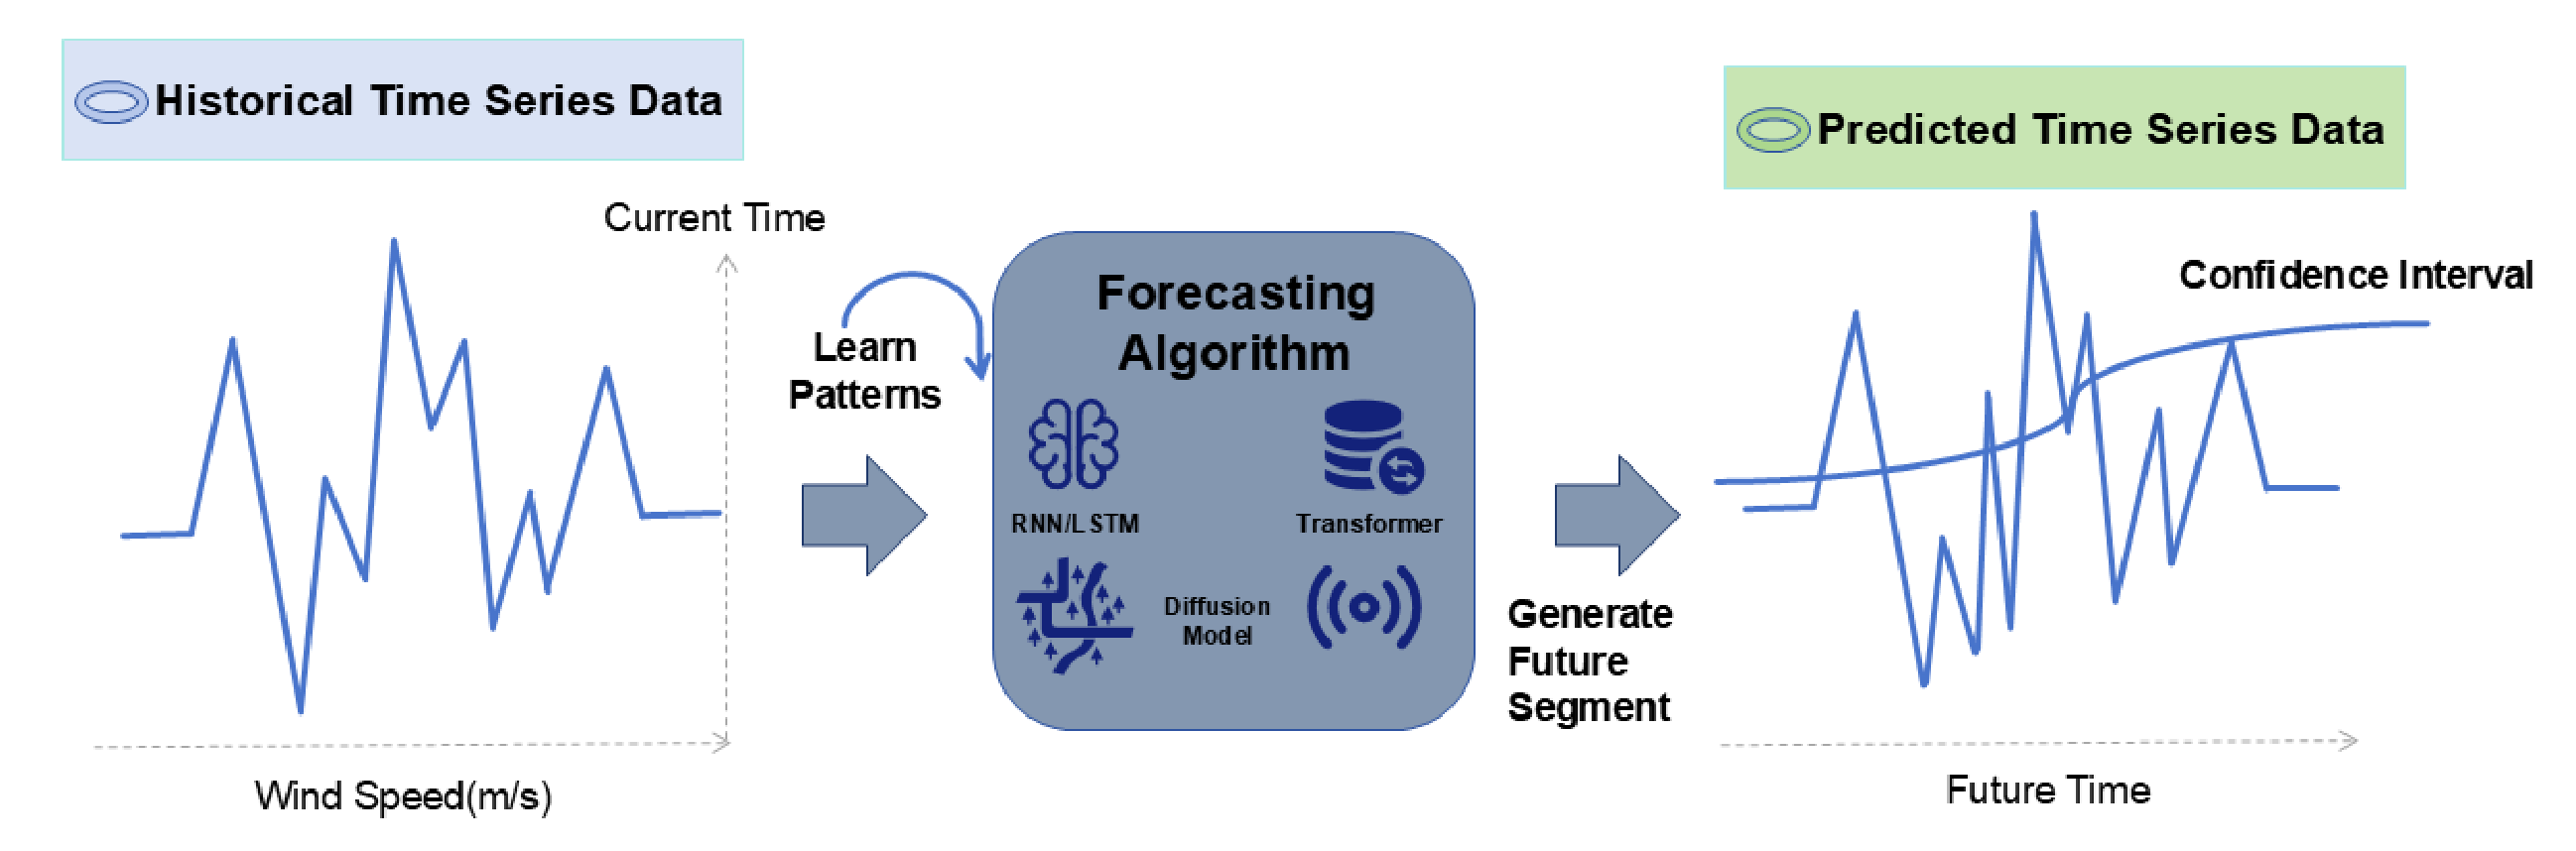
\includegraphics[width=0.9\linewidth]{figures/figure2.eps}
% \caption{Time Series Forecast}
% \label{fig:qualitative}
% \end{figure*}

\subsection{Statistical Modeling}
Classical forecasting relied on explicit statistical assumptions, with linear models dominating the field. 
The Autoregressive Integrated Moving Average (ARIMA)~\cite{DBLP:conf/nips/NaimanBPAFA24} and its seasonal variant SARIMA provided interpretable formulations under stationarity assumptions, while Vector Autoregression (VAR)~\cite{Zivot2003} extended these ideas to multivariate settings. 
Nonparametric methods like Holt–Winters exponential smoothing~\cite{KOEHLER2001269} and the Error–Trend–Seasonality (ETS) framework~\cite{RePEc2009} modeled trend-seasonality interactions without strict distributional requirements. 
From a probabilistic perspective, Gaussian Processes (GPs)~\cite{2005Gaussian} introduced Bayesian inference for time series, providing principled uncertainty quantification via kernel functions.

% However, these methods often struggle with the nonlinear, nonstationary, and high-dimensional dynamics prevalent in modern applications due to their reliance on fixed functional forms and limited scalability.

\subsection{Deep Learning Revolution}
Neural networks revolutionized forecasting by enabling hierarchical feature learning and nonlinear modeling. 
Early recurrent architectures like LSTM~\cite{HSJ1997} and GRU~\cite{2014Learning} addressed gradient issues to capture long-term dependencies, with DeepAR~\cite{2020DeepAR} establishing a deep probabilistic framework. 
Convolution-based models such as WaveNet~\cite{2016WaveNet} and TCNs~\cite{DBLP:conf/iclr/BaiKK19} overcame sequential bottlenecks using dilated causal convolutions for efficient parallel processing. 
More recently, attention-based architectures like the Transformer~\cite{2017Attention}, Informer~\cite{2020Informer}, and Autoformer~\cite{2021Autoformer} have become dominant by capturing global temporal dependencies through self-attention and frequency-domain analysis.

\subsection{Emerging Diffusion Paradigm}
Diffusion models have recently emerged as powerful generative tools for time series.
TimeGrad~\cite{2021Autoregressive} introduced autoregressive denoising diffusion for probabilistic forecasting, while CSDI~\cite{2021CSDI} extended this to conditional score-based diffusion for imputation tasks. 
To improve efficiency and handle long sequences, SSSD~\cite{alcaraz2022diffusion} incorporated state space models, and TSDiff~\cite{kollovieh2023predict} proposed 2D representations to accommodate variable-length sequences. 
Spatial-temporal extensions like DiffSTG~\cite{wen2023DiffSTG} embedded graph structures to model complex spatio-temporal dynamics. 
% \subsection{Statistical Modeling}
% Early approaches to time series forecasting primarily relied on explicit statistical assumptions about temporal dependencies and noise distributions.

% Linear models such as the Autoregressive Integrated Moving Average (ARIMA) model~\cite{2013ARIMA} have long dominated classical forecasting, offering interpretable formulations under stationarity and linearity assumptions. Its seasonal variant, SARIMA, further extends the framework to capture periodic fluctuations. The Vector Autoregression (VAR) model~\cite{Zivot2003} generalizes these ideas to the multivariate setting, enabling linear inter-series dependency modeling across multiple correlated variables.

% Beyond parametric formulations, nonparametric smoothing methods such as the Holt–Winters exponential smoothing~\cite{KOEHLER2001269} empirically model trend–seasonality interactions without requiring strong distributional assumptions. The Error–Trend–Seasonality (ETS) framework~\cite{RePEc2009} unifies these techniques by decomposing time series into interpretable components under a state-space representation, supporting both additive and multiplicative structures.

% From a probabilistic perspective, Gaussian Process (GP) models~\cite{2005Gaussian} introduced a Bayesian approach to time series prediction, providing principled uncertainty quantification through kernel-based covariance functions. These models capture local smoothness and uncertainty propagation effectively in low-dimensional settings.


% However, despite their interpretability and strong theoretical grounding, these statistical methods struggle to model nonlinear, nonstationary, and high-dimensional temporal dynamics common in modern real-world applications.Their reliance on fixed functional forms and limited scalability restricts their ability to capture complex dependencies and long-range interactions, motivating the transition toward deep learning and generative paradigms in subsequent research.

% \subsection{Deep Learning Revolution}
% The emergence of neural networks has fundamentally transformed time series forecasting by enabling hierarchical feature learning and nonlinear temporal dependency modeling. Unlike statistical approaches with fixed assumptions, neural networks learn dynamic representations directly from data, capturing complex interactions across multiple time scales.

% Early sequential architectures such as the Long Short-Term Memory (LSTM) network~\cite{HSJ1997} addressed the vanishing gradient problem through gated mechanisms that preserve long-term information, while the Gated Recurrent Unit (GRU)~\cite{2014Learning} simplified this structure to enhance computational efficiency with comparable accuracy. Building on these foundations, DeepAR~\cite{2020DeepAR} combined autoregressive likelihood estimation with LSTM encoders, establishing a deep probabilistic framework for multivariate time series forecasting.

% To overcome the sequential bottleneck of recurrent networks, convolution-based models such as WaveNet~\cite{2016WaveNet} and Temporal Convolutional Networks (TCNs)~\cite{DBLP:conf/iclr/BaiKK19} employed dilated causal convolutions and residual connections to capture long-range dependencies in a fully parallelizable manner. These architectures marked a shift from sequential recurrence to efficient hierarchical temporal modeling.

% More recently, attention-based architectures have advanced forecasting by modeling global temporal dependencies. The Transformer~\cite{2017Attention} introduced self-attention to directly capture long-range interactions, achieving strong performance across diverse sequence tasks. Its variants, Informer~\cite{2020Informer} and Autoformer~\cite{2021Autoformer}, further improved efficiency and interpretability through sparse attention and frequency-domain autocorrelation, respectively, making attention mechanisms a dominant paradigm in long-horizon time series forecasting.

% %\subsection{Diffusion Models in Time Series}
% \subsection{Emerging Diffusion Paradigm}
% Building on deep learning successes, diffusion models have emerged as powerful generative tools:recent research has shifted toward generative frameworks that model the full predictive distribution of time series rather than point estimates. TimeGrad~\cite{2021Autoregressive} first introduced autoregressive denoising diffusion for multivariate probabilistic forecasting, demonstrating the ability of diffusion models to capture uncertainty through iterative noise refinement. CSDI~\cite{2021CSDI} extended this idea with conditional score-based diffusion, enabling flexible handling of missing observations and context-aware forecasting. For efficient long-range sequence modeling, SSSD~\cite{alcaraz2022diffusion} incorporated state space models into the diffusion framework, addressing the computational challenges of capturing long-term dependencies. TSDiff~\cite{naiman_utilizing_nodate} proposed a novel approach by encoding variable -length time series into 2D representations to accommodate the flexibility of sequence lengths. To handle spatio-temporal data, DiffSTG~\cite{wen2023DiffSTG} embedded graph structures into diffusion models, enabling effective modeling of both spatial correlations and temporal dynamics.Subsequent methods incorporated learned guidance, hybrid backbones, and structured state-space formulations to improve sampling efficiency and capture long-range temporal dependencies.
%\vspace{-15pt}
% \begin{table}[htbp]
% \caption{Comparison of Different Time-Series Methods}
% \label{tab:model_comparison}
% \begin{tabular}{@{}lcc@{}}
% \toprule
% \textbf{Method} & \textbf{Var.-Len.} & \textbf{Multi-Scale} \\
% \midrule
% \multicolumn{3}{@{}l}{\textit{Traditional Statistical}} \\
% \quad ARIMA/SARIMA~\cite{2013ARIMA} & $\times$ & $\times$ \\
% \quad VAR~\cite{Zivot2003}            & $\times$ & $\times$ \\
% \quad Holt-Winters~\cite{KOEHLER2001269}   & $\times$ & $\times$ (seasonal) \\
% \quad ETS~\cite{RePEc2009}~\cite{2005Gaussian} & $\checkmark$ & $\times$ \\
% \quad Gaussian Process~\cite{2005Gaussian} & $\checkmark$ & $\times$ \\
% \midrule
% \multicolumn{3}{@{}l}{\textit{Deep Learning}} \\
% \quad LSTM/GRU~\cite{HSJ1997,2014Learning}       & \checkmark & $\times$ \\
% \quad DeepAR~\cite{2020DeepAR}         & $\times$ & $\times$ \\
% \quad WaveNet/TCN~\cite{2016WaveNet,DBLP:conf/iclr/BaiKK19}    & \checkmark & \checkmark$^\dag$ \\
% \quad Transformer~\cite{2017Attention}    & \checkmark & $\times$ \\
% \quad Informer~\cite{2020Informer}       & \checkmark & $\times$ \\
% \quad Autoformer~\cite{2021Autoformer}     & \checkmark & \checkmark$^\dag$ \\
% \midrule
% \multicolumn{3}{@{}l}{\textit{Diffusion Models}} \\
% \quad TimeGrad~\cite{2021Autoregressive}       & $\times$ & $\times$ \\
% \quad CSDI~\cite{2021CSDI}           & $\times$ & $\times$ \\
% \quad SSSD~\cite{alcaraz2022diffusion}            & \checkmark & $\times$ \\
% \quad TSDiff~\cite{kollovieh2023predict}          & \checkmark & $\times$ \\
% \quad DiffSTG~\cite{wen2023DiffSTG}         & $\times$ & $\times$ \\
% \quad \textbf{Our Method} & $\boldsymbol{\checkmark}$ & $\boldsymbol{\checkmark}$ \\ 
% \bottomrule
% \smallskip
% {\small $^\dag$ Depends on dilation / seasonal decomposition}
% \end{tabular}
% \end{table}


% \subsubsection{Foundational Works}
% \begin{itemize}
% 	\item TimeGrad \cite{2021Autoregressive} combined diffusion with RNN-based conditioning
% 	\item CSDI \cite{2021CSDI} adapted score-based diffusion for missing value imputation
% \end{itemize}

% \subsubsection{Architectural Innovations}
% Recent advances address key limitations:
% \begin{itemize}
% 	\item SSSD \cite{alcaraz2022diffusion} integrated state space models for efficient long-range modeling
% 	\item TSDiff \cite{naiman_utilizing_nodate} encoded variable-length series as 2D representations
% 	\item DiffSTG \cite{10.1145/3589132.3625614} incorporated graph structures for spatio-temporal data
% 	\item mr-Diff \cite{shen_multi-resolution_2024} pioneered multi-scale decomposition via seasonal-trend analysis
% \end{itemize}


%\vspace{-15pt}


% \textbf{Critical Gap:} Existing diffusion approaches exhibit three key limitations,which reflected in the %\autoref{tab:model_comparison}: 
% (1) rigidity in handling variable-length inputs, 
% (2) absence of explicit multi-scale modeling, and 
% (3) computational inefficiency in inference. 

% Our framework tackles these challenges through three core design principles. First, we introduce an adaptive delay embedding mechanism that effectively handles variable-length input sequences by dynamically adjusting the temporal context window. Second, we employ a hierarchical multi-resolution decomposition strategy to capture and model temporal patterns across multiple time scales—ranging from fine-grained fluctuations to long-term trends. Third, we propose a conditionally guided diffusion process, which leverages coarse-level trend information as structural priors to guide the generative refinement, thereby significantly improving both computational efficiency and training stability. Together, these components enable our model to robustly learn complex temporal dynamics while maintaining scalability and generalization across diverse forecasting scenarios.
Our framework addresses these exsiting challenges through three core innovations: an adaptive delay embedding mechanism for handling variable-length sequences, a hierarchical multi-resolution decomposition strategy to capture multi-scale temporal patterns, and a conditionally guided diffusion process that leverages coarse-level trends as structural priors. Together, these components ensure robust learning of complex dynamics while enhancing computational efficiency and training stability.










